\section{Global theory of plane curves}

The global theory is related to ``topology'' of the geometric objects.
For 1-dimensional geometry, \ie\ curves, it's always oriented. And the simplest distinction in topology
is ``open'' and ``closed''.

\begin{definition}[Closed curves]
    \begin{itemize}\hfill
        \item We say
              \(\alpha\colon I=[a,b]\to \mathbb{R}
              ^3\)
              (or \(\mathbb{R}^2\))
              is a closed regular curve, if
              \(\alpha(a)=\alpha(b)\)
              and
              \(\alpha^{(k)}
              (a)=\alpha^{(k)}(b)\)
              (in another word,
              \(\alpha\colon \mathbb{S}^1\to \mathbb{R}^3\)
              is a differentiable curve).
        \item Furthermore, if
              \(\alpha\)
              has no
              self-intersection point other than
              $\alpha(a)=\alpha(b)$,
              then we call $\alpha(s)$ to be a simple closed curve.
    \end{itemize}
\end{definition}
\begin{center}
    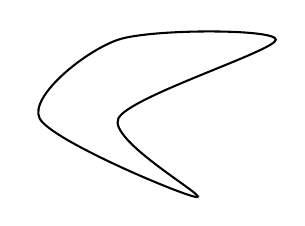
\begin{tikzpicture}
        \draw plot [smooth cycle] coordinates {(0,0) (1,1) (3,1) (1,0) (2,-1)};
    \end{tikzpicture}
\end{center}

\subsection{Isoperimetric inequality}
This is one of the oldest and most famous problem in geometry. It's still attracting mathematicians to investigate such problem in various geometric formulations nowadays.
\begin{question}
    Given a closed plane curve \(C\) with. Let \(D\) be the
    region bounded by \(C\). When does the region have the
    maximal area, if \(C\) is among all the curves with
    fixed length?
\end{question}
\begin{answer}
    \(C\) must be a circle when the maximal area is
    achieved.
\end{answer}
\begin{remark}
    Even though we'll only handle smooth, simple closed
    curves in the following discussion, in general we
    don't have to assume the curve to be simple:
    {\ooalign{$\bigcirc $\cr $\ \ \,\bigcirc $}}
    has less area than $\bigcirc $.(caution: their boundaries are intended to have the same length). Thick about how
        {\ooalign{$\bigcirc $\cr $\ \ \,\bigcirc $}}
    comes from $\bigcirc $.
\end{remark}

\subsubsection*{Proofs of the Isoperimetric inequality}
\begin{proof}1 (Hurwitz's proof) This relies on the ``Wirtinger's inequality''.

    Let $\alpha(t)$ be a closed, simple smooth curve, where $t$ can be any parameter. The length of it is
    \[L=\int_a^b\sqrt{x'(t)^2+y'(t)^2}\dd t.\]

    Observe that we need to find the lower bound of $L^2$.
    Generally, for an integral $L=\int \sqrt{f}\dd t$, H\"older
    inequality (or Cauchy-Schwarz) naturally gives estimate of
    L. Hence, it's natural to find a ``good parameter'' to
    clear. Although the arclength $s$ is a good candidate, it
    turns out in this case that another good parameter is
    \[\theta=\frac{2\pi}{L}s.\]
    $s\in [0,L]\Rightarrow \theta \in [0,2\pi]$.
    (This parameter $\theta$ comes from the ``Wirtinger's inequality', but of course a rescaling of wirtinger's inequality allows us to use $s$ as usual).

    Let's take $\theta=\frac{2\pi}{L}s$, then
    \[\left(\frac{\dd x}{\dd \theta}\right)^2+\left(\frac{\dd y}{\dd \theta}\right)^2=\left(\left(\frac{\dd x}{\dd s}\right)^2+\left(\frac{\dd y}{\dd s}\right)^2\right)\left(\frac{\dd s}{\dd \theta}\right)^2=\left(\frac{L}{2\pi}\right)^2.\]
    \[\Rightarrow \frac{L^2}{2\pi}=\frac{L^2}{4\pi^2}\cdot 2\pi=\int_0^{2\pi}\left(x'(\theta)^2+y'(\theta)^2\right)\dd \theta.\]
    Therefore,
    \begin{align}
        2\left(\frac{L^2}{4\pi}-A\right) & =\int_0^{2\pi}\left(x'(\theta)^2+y'(\theta)^2\right)\dd \theta-2\int_0^{2\pi}x(\theta)y'(\theta)\dd \theta \notag \\
                                         & =\int_0^{2\pi}x'(\theta)^2-x(\theta)^2+\underbrace{(y'(\theta)-x(\theta))^2}_{\ge 0}\dd \theta \notag             \\
                                         & \ge \int_0^{2\pi}x'(\theta)^2-x(\theta)^2 \dd \theta \tag{$\bigstar$}
        .\end{align}
    Now, the proof reduces to the following lemma.

    \begin{lemma}[Wirtinger's inequality]
        Let $f\colon\mathbb{R}\to \mathbb{R}$ be a $2\pi$-periodic smooth
        function and $\int_0^{2\pi}f(\theta)\dd \theta=0$, Then
        \[\int_0^{2\pi}f(\theta)^2\dd \theta\le \int_0^{2\pi}f'(\theta)^2\dd \theta,\]
        and equality holds iff $f(\theta)=a\cos(\theta)+b\sin(\theta)$.
    \end{lemma}
    (Proof of the lemma is left as a homework problem.)

    To apply this to $(\bigstar)$, we need to assume $\int_0^{2\pi}x(\theta)\dd \theta=0$. However, we know the center of mass of the curve is $\left(\frac{\int x(\theta)\dd \theta}{L},\frac{\int y(\theta)\dd \theta}{L}\right)$, and by choosing the origin of $\mathbb{R}^2$ as the center of mass, we can guarantee $\int_0^{2\pi}x(\theta)\dd \theta=0$, this yields $\bigstar\ge 0$, \ie\ $L^2\ge 4\pi A$. Moreover, equality implies
    \[x(\theta)=a\cos(\theta)+b\sin(\theta)\text{ and }y'(\theta)=x(\theta)\Rightarrow\]
    \[y(\theta)=a\sin(\theta)-b\cos(\theta)+c.\]
    So $(x(\theta),y(\theta))$ is a circle.
\end{proof}
\begin{proof}2 (By Schmidt)
    See Do Carmo's book (page 33-35). It will be lectured by TA in a recitation.
\end{proof}
\begin{remark}\hfill
    \begin{enumerate}[(1)]
        \item There are many other proofs of Isoperimetric
              inequality. In the homework 3, we will use a
              modern tool-curve shortening flow to give a proof.
        \item
              \begin{align*}
                  L^2                                                                                & \ge 4 \pi A  \Rightarrow \frac{L^2}{4\pi}\ge A \Rightarrow
                  \frac{L^2}{4\pi^2 r^2}\ge \frac{A}{\pi r^2}(\text{take }r=1)                                                                                    \\
                  \Rightarrow \frac{L}{2\pi}\ge \left(\frac{A}{\pi}\right)^{\frac{1}{2}}\text{\ie\ } &
                  \frac{\text{length of curve}}{\text{length of the unit circle}}
                  \ge \left(\frac{\text{Area bounded by the curve}}{\text{Area of the unit disk}}\right)^{\frac{1}{2}}
                  .\end{align*}
    \end{enumerate}
\end{remark}
$\bullet$ \textbf{Generalization}: Let $E$ be a compact domain in $\mathbb{R}^n$ with smooth boundary $\partial E$, then
\[
    \frac{\text{Area}(\partial E)}{\text{Area of the unit sphere in }\mathbb
        {R}^n}\ge \left(\frac{\text{Volume of }E}{\text{Volume of the unit
            ball}}\right)^{\frac{n-1}{n}}
\]
For simplicity, we write
\[
    \frac{|\partial E|}{\partial B^n} \ge \left(\frac{|E|}{|B^n|}\right)^
    {\frac{n-1}{n}}.
\]
\begin{question}
    Can you propose some generalizations of isoperimetric inequality?
    Isoperimetric inequality is one of the motivation to develop geometric measure theory!
\end{question}
\subsection{Four-vertex theorem}
\begin{theorem}\label{thm:four-vertex theorem}
    A simple closed convex plane curve has at least four vertices.
\end{theorem}
\begin{remark}
    The four-vertex theorem holds also for simple closed non-convex curves.
    The proof is harder, however.
\end{remark}
\begin{definition}[Convex curves]
    $\alpha(s)$ is a convex curve, if at each point $\alpha(s_0)$, the whole curve lies on the same side of the tangent line.
\end{definition}




\tikzset{every picture/.style={line width=0.75pt}} %set default line width to 0.75pt        

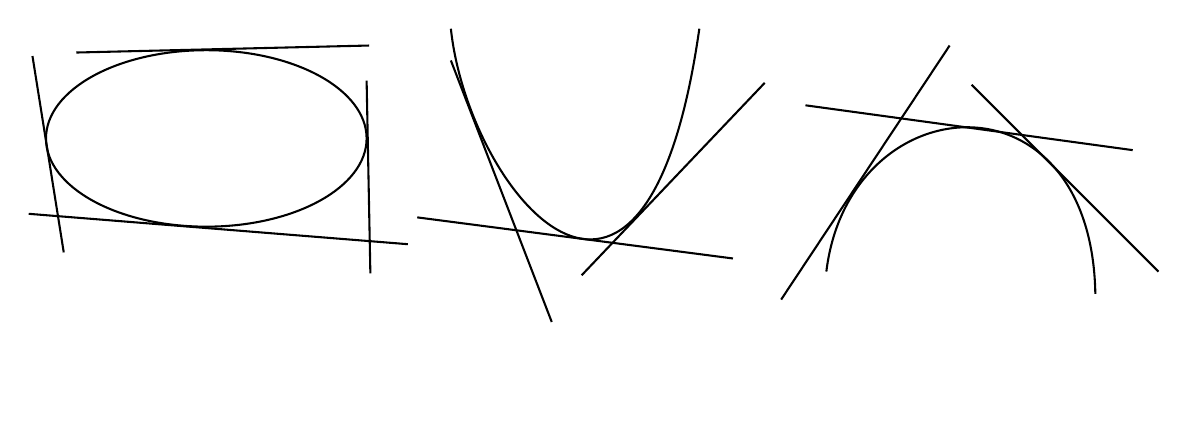
\begin{tikzpicture}[x=0.75pt,y=0.75pt,yscale=-0.9,xscale=0.9]
    %uncomment if require: \path (0,300); %set diagram left start at 0, and has height of 300

    %Shape: Ellipse [id:dp6953189046620603] 
    \draw   (48.45,88.74) .. controls (48.45,62.65) and (86.87,41.5) .. (134.27,41.5) .. controls (181.67,41.5) and (220.09,62.65) .. (220.09,88.74) .. controls (220.09,114.83) and (181.67,135.97) .. (134.27,135.97) .. controls (86.87,135.97) and (48.45,114.83) .. (48.45,88.74) -- cycle ;
    %Straight Lines [id:da8702738615642636] 
    \draw    (220.09,57.77) -- (222.1,161) ;
    %Straight Lines [id:da3706263383184776] 
    \draw    (64.66,42.75) -- (221.43,39) ;
    %Straight Lines [id:da3054598329478624] 
    \draw    (39.2,129.09) -- (242.2,145.36) ;
    %Straight Lines [id:da15509227924350344] 
    \draw    (41.21,44.63) -- (57.96,149.74) ;
    %Curve Lines [id:da726485353707341] 
    \draw    (265.2,30) .. controls (274.4,117) and (369.2,233) .. (398.2,30) ;
    %Straight Lines [id:da03667314517418263] 
    \draw    (265.2,47) -- (319.2,187) ;
    %Straight Lines [id:da7191564753420123] 
    \draw    (247.2,131) -- (416.2,153) ;
    %Straight Lines [id:da8951764820712218] 
    \draw    (433.2,59) -- (335.2,162) ;
    %Curve Lines [id:da7789942846266422] 
    \draw    (466.2,160) .. controls (478.4,60) and (608.2,50) .. (610.2,172) ;
    %Straight Lines [id:da306587637969457] 
    \draw    (455,71) -- (630.2,95) ;
    %Straight Lines [id:da1811450298421866] 
    \draw    (532.2,39) -- (442,175) ;
    %Straight Lines [id:da35817044779115514] 
    \draw    (544,60) -- (644,160) ;

\end{tikzpicture}
The convex curve has the following useful characterization.
\begin{proposition}
    $\alpha(s)$ is a convex curve $\Leftrightarrow $ at each point $\alpha(s_0)$, only one of the following holds:
    \begin{quotation}
        For all $s\in I$, either $(\alpha(s)-\alpha(s_0))\cdot \vec{n}(s_0)\ge 0$ or $(\alpha(s)-\alpha(s_0))\cdot \vec{n}(s_0)\le 0$.
    \end{quotation}
    Geometrically, this means at a convex point, the angle between vector $\alpha(s)-\alpha(s_0)$ and $\vec{n}(s_0)$ should be either $[0,\frac{\pi}{2}]$ or $[\pi,\frac{3\pi}{2}]$.
\end{proposition}
\begin{example}\hfill

    \tikzset{every picture/.style={line width=0.75pt}} %set default line width to 0.75pt        

    \begin{center}
        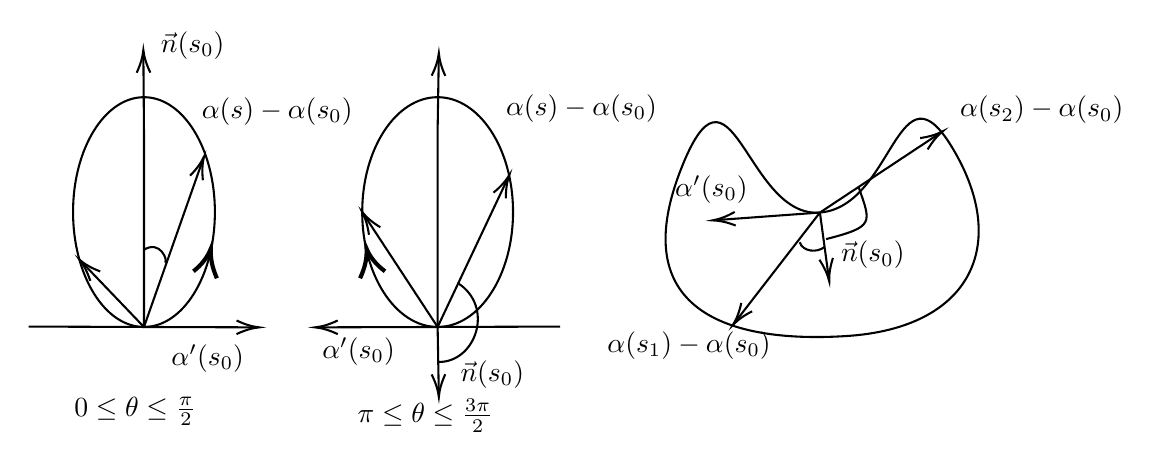
\begin{tikzpicture}[x=0.75pt,y=0.75pt,yscale=-1,xscale=1]
            %uncomment if require: \path (0,300); %set diagram left start at 0, and has height of 300

            %Shape: Ellipse [id:dp7591861540053348] 
            \draw   (52.86,98.9) .. controls (52.86,68.33) and (68.16,43.55) .. (87.03,43.55) .. controls (105.9,43.55) and (121.2,68.33) .. (121.2,98.9) .. controls (121.2,129.48) and (105.9,154.26) .. (87.03,154.26) .. controls (68.16,154.26) and (52.86,129.48) .. (52.86,98.9) -- cycle ;
            %Straight Lines [id:da06336028525669235] 
            \draw    (31.5,154.07) -- (140.55,154.44) ;
            \draw [shift={(142.55,154.45)}, rotate = 180.19] [color={rgb, 255:red, 0; green, 0; blue, 0 }  ][line width=0.75]    (10.93,-3.29) .. controls (6.95,-1.4) and (3.31,-0.3) .. (0,0) .. controls (3.31,0.3) and (6.95,1.4) .. (10.93,3.29)   ;
            %Straight Lines [id:da8240848008506814] 
            \draw    (87.03,154.26) -- (115.29,74.05) ;
            \draw [shift={(115.95,72.17)}, rotate = 109.41] [color={rgb, 255:red, 0; green, 0; blue, 0 }  ][line width=0.75]    (10.93,-3.29) .. controls (6.95,-1.4) and (3.31,-0.3) .. (0,0) .. controls (3.31,0.3) and (6.95,1.4) .. (10.93,3.29)   ;
            %Straight Lines [id:da8702455490360739] 
            \draw    (87.03,154.26) -- (87.03,59.36) -- (86.74,22.8) ;
            \draw [shift={(86.73,20.8)}, rotate = 89.55] [color={rgb, 255:red, 0; green, 0; blue, 0 }  ][line width=0.75]    (10.93,-3.29) .. controls (6.95,-1.4) and (3.31,-0.3) .. (0,0) .. controls (3.31,0.3) and (6.95,1.4) .. (10.93,3.29)   ;
            %Straight Lines [id:da8932284835920707] 
            \draw    (87.03,154.26) -- (57.39,123.32) ;
            \draw [shift={(56,121.88)}, rotate = 46.23] [color={rgb, 255:red, 0; green, 0; blue, 0 }  ][line width=0.75]    (10.93,-3.29) .. controls (6.95,-1.4) and (3.31,-0.3) .. (0,0) .. controls (3.31,0.3) and (6.95,1.4) .. (10.93,3.29)   ;
            \draw  [line width=1.5]  (110.87,127.44) .. controls (114.91,124.19) and (117.7,120.57) .. (119.23,116.56) .. controls (118.95,120.94) and (119.93,125.68) .. (122.16,130.8) ;
            %Shape: Ellipse [id:dp3057067643925675] 
            \draw   (264.85,98.9) .. controls (264.85,68.33) and (248.58,43.55) .. (228.51,43.55) .. controls (208.45,43.55) and (192.18,68.33) .. (192.18,98.9) .. controls (192.18,129.48) and (208.45,154.26) .. (228.51,154.26) .. controls (248.58,154.26) and (264.85,129.48) .. (264.85,98.9) -- cycle ;
            %Straight Lines [id:da7048479708357958] 
            \draw    (287.55,154.07) -- (171.47,154.44) ;
            \draw [shift={(169.47,154.45)}, rotate = 359.82] [color={rgb, 255:red, 0; green, 0; blue, 0 }  ][line width=0.75]    (10.93,-3.29) .. controls (6.95,-1.4) and (3.31,-0.3) .. (0,0) .. controls (3.31,0.3) and (6.95,1.4) .. (10.93,3.29)   ;
            %Straight Lines [id:da9292206875165037] 
            \draw    (228.51,154.26) -- (262.22,82.86) ;
            \draw [shift={(263.07,81.05)}, rotate = 115.27] [color={rgb, 255:red, 0; green, 0; blue, 0 }  ][line width=0.75]    (10.93,-3.29) .. controls (6.95,-1.4) and (3.31,-0.3) .. (0,0) .. controls (3.31,0.3) and (6.95,1.4) .. (10.93,3.29)   ;
            %Straight Lines [id:da8265464948656487] 
            \draw    (228.51,154.26) -- (228.51,59.36) -- (229.07,24.31) ;
            \draw [shift={(229.1,22.31)}, rotate = 90.91] [color={rgb, 255:red, 0; green, 0; blue, 0 }  ][line width=0.75]    (10.93,-3.29) .. controls (6.95,-1.4) and (3.31,-0.3) .. (0,0) .. controls (3.31,0.3) and (6.95,1.4) .. (10.93,3.29)   ;
            %Straight Lines [id:da8724360322486144] 
            \draw    (228.51,154.26) -- (193.28,100.58) ;
            \draw [shift={(192.18,98.9)}, rotate = 56.72] [color={rgb, 255:red, 0; green, 0; blue, 0 }  ][line width=0.75]    (10.93,-3.29) .. controls (6.95,-1.4) and (3.31,-0.3) .. (0,0) .. controls (3.31,0.3) and (6.95,1.4) .. (10.93,3.29)   ;
            \draw  [line width=1.5]  (203.16,127.44) .. controls (198.86,124.19) and (195.9,120.57) .. (194.28,116.56) .. controls (194.56,120.94) and (193.53,125.68) .. (191.15,130.8) ;
            %Straight Lines [id:da3485129106090552] 
            \draw    (228.51,154.26) -- (229.07,186) ;
            \draw [shift={(229.1,188)}, rotate = 269] [color={rgb, 255:red, 0; green, 0; blue, 0 }  ][line width=0.75]    (10.93,-3.29) .. controls (6.95,-1.4) and (3.31,-0.3) .. (0,0) .. controls (3.31,0.3) and (6.95,1.4) .. (10.93,3.29)   ;
            %Shape: Polygon Curved [id:ds10755820169219077] 
            \draw   (345.25,79.55) .. controls (369.98,14.77) and (376.88,101.99) .. (412.7,99.13) .. controls (448.52,96.27) and (450.16,23.06) .. (477.14,69) .. controls (504.12,114.95) and (485.38,154.86) .. (425.44,158.63) .. controls (365.49,162.4) and (320.53,144.32) .. (345.25,79.55) -- cycle ;
            %Straight Lines [id:da35610041851976515] 
            \draw    (412.7,99.13) -- (362.99,102.75) ;
            \draw [shift={(360.99,102.9)}, rotate = 355.83] [color={rgb, 255:red, 0; green, 0; blue, 0 }  ][line width=0.75]    (10.93,-3.29) .. controls (6.95,-1.4) and (3.31,-0.3) .. (0,0) .. controls (3.31,0.3) and (6.95,1.4) .. (10.93,3.29)   ;
            %Straight Lines [id:da6090255533817175] 
            \draw    (412.7,99.13) -- (416.92,130.29) ;
            \draw [shift={(417.19,132.27)}, rotate = 262.27] [color={rgb, 255:red, 0; green, 0; blue, 0 }  ][line width=0.75]    (10.93,-3.29) .. controls (6.95,-1.4) and (3.31,-0.3) .. (0,0) .. controls (3.31,0.3) and (6.95,1.4) .. (10.93,3.29)   ;
            %Straight Lines [id:da9846059751183915] 
            \draw    (412.7,99.13) -- (371.96,151.78) ;
            \draw [shift={(370.73,153.36)}, rotate = 307.73] [color={rgb, 255:red, 0; green, 0; blue, 0 }  ][line width=0.75]    (10.93,-3.29) .. controls (6.95,-1.4) and (3.31,-0.3) .. (0,0) .. controls (3.31,0.3) and (6.95,1.4) .. (10.93,3.29)   ;
            %Straight Lines [id:da9899745827591568] 
            \draw    (412.7,99.13) -- (470.23,61.07) ;
            \draw [shift={(471.9,59.96)}, rotate = 146.51] [color={rgb, 255:red, 0; green, 0; blue, 0 }  ][line width=0.75]    (10.93,-3.29) .. controls (6.95,-1.4) and (3.31,-0.3) .. (0,0) .. controls (3.31,0.3) and (6.95,1.4) .. (10.93,3.29)   ;
            %Curve Lines [id:da7720258932280717] 
            \draw    (86.73,117.21) .. controls (94.97,111.93) and (98.72,122.48) .. (97.22,123.23) ;
            %Curve Lines [id:da3500113291593643] 
            \draw    (228.81,171.13) .. controls (247.09,171.43) and (256.08,144.32) .. (238.1,133.02) ;
            %Curve Lines [id:da041829079173997474] 
            \draw    (402.96,113.44) .. controls (404.45,117.96) and (411.2,118.71) .. (414.94,115.7) ;
            %Curve Lines [id:da01241211464079428] 
            \draw    (415.69,111.93) .. controls (438.92,105.91) and (437.43,104.4) .. (431.43,87.08) ;

            % Text Node
            \draw (98.78,161.33) node [anchor=north west][inner sep=0.75pt]    {$\alpha '( s_{0})$};
            % Text Node
            \draw (113.4,42.15) node [anchor=north west][inner sep=0.75pt]    {$\alpha ( s) -\alpha ( s_{0})$};
            % Text Node
            \draw (51.95,186.49) node [anchor=north west][inner sep=0.75pt]    {$0\leq \theta \leq \frac{\pi }{2}$};
            % Text Node
            \draw (171.47,157.85) node [anchor=north west][inner sep=0.75pt]    {$\alpha '( s_{0})$};
            % Text Node
            \draw (260.02,40.68) node [anchor=north west][inner sep=0.75pt]    {$\alpha ( s) -\alpha ( s_{0})$};
            % Text Node
            \draw (93.72,10.56) node [anchor=north west][inner sep=0.75pt]    {$\vec{n}( s_{0})$};
            % Text Node
            \draw (238.06,169.13) node [anchor=north west][inner sep=0.75pt]    {$\vec{n}( s_{0})$};
            % Text Node
            \draw (188.45,187.51) node [anchor=north west][inner sep=0.75pt]    {$\pi \leq \theta \leq \frac{3\pi }{2}$};
            % Text Node
            \draw (341.49,79.86) node [anchor=north west][inner sep=0.75pt]    {$\alpha '( s_{0})$};
            % Text Node
            \draw (421.4,111.4) node [anchor=north west][inner sep=0.75pt]    {$\vec{n}( s_{0})$};
            % Text Node
            \draw (308.84,155.08) node [anchor=north west][inner sep=0.75pt]    {$\alpha ( s_{1}) -\alpha ( s_{0})$};
            % Text Node
            \draw (478.76,41.59) node [anchor=north west][inner sep=0.75pt]    {$\alpha ( s_{2}) -\alpha ( s_{0})$};

        \end{tikzpicture}
    \end{center}
\end{example}
\begin{example}
    $\alpha(t)=\left((1+2\cos t)\cos t,(1+2\cos t)\sin t\right),~ t\in \mathbb{R}.$

    \begin{center}
        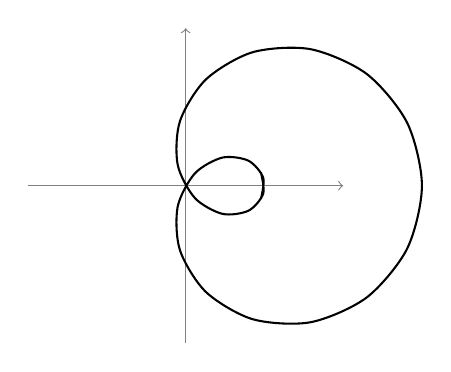
\begin{tikzpicture}
            \draw[black!50, thin, ->] (0, -2) -- (0, 2) ;
            \draw[black!50, thin, ->] (-2, 0) -- (2, 0) ;
            \draw[smooth,domain=-190:190,variable=\t]
            plot ({(1+2*cos(\t))*cos(\t)},{(1+2*cos(\t))*sin(\t)});
        \end{tikzpicture}
    \end{center}
\end{example}
\begin{proposition}
    \label{week3_prop2}
    $\alpha(s)$ is a simple closed curve, then
    \begin{center}
        $\alpha(s)$ is convex $\Leftrightarrow $ $k(s)\ge 0~\forall s$ or $k(s)\le 0~\forall s$.
    \end{center}
\end{proposition}
Previously, we have seen that $k(s)$ measures the rate of change
of the angle between tangent vectors. Let's see another similar application.
Let $\alpha(s)$ be parametrized by arclength, then $t(s)\equiv\alpha'(s)$
is a unit tangent vector, \ie\ $|t(s)|=1$.
\begin{center}



    \tikzset{every picture/.style={line width=0.75pt}} %set default line width to 0.75pt        

    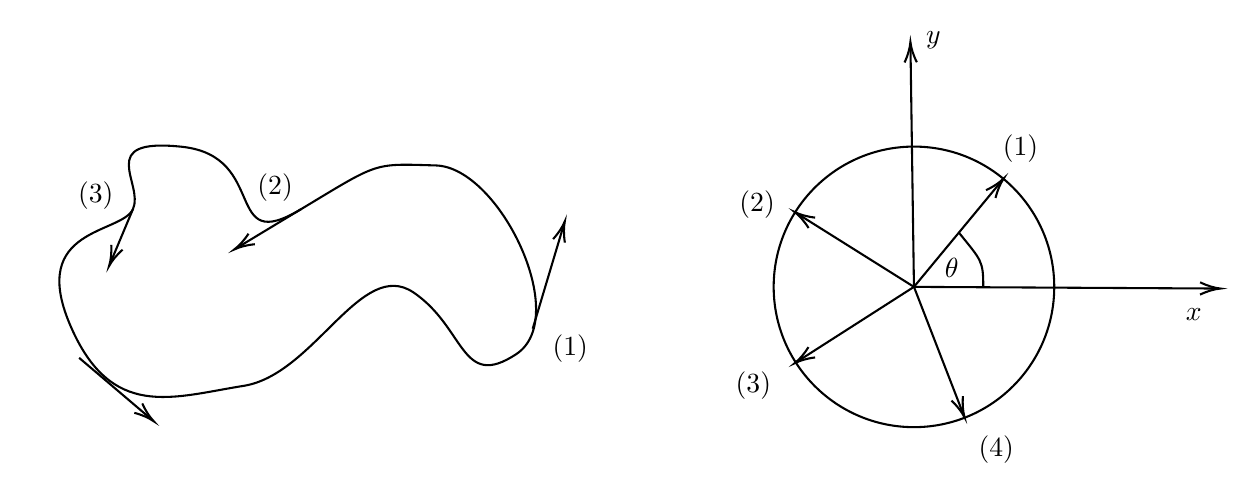
\begin{tikzpicture}[x=0.75pt,y=0.75pt,yscale=-0.9,xscale=0.9]
        %uncomment if require: \path (0,300); %set diagram left start at 0, and has height of 300

        %Shape: Polygon Curved [id:ds0026171910463155257] 
        \draw   (73,110) .. controls (79.2,96.6) and (52.2,71.6) .. (99.2,76.6) .. controls (146.2,81.6) and (120.8,135.4) .. (163,110) .. controls (205.2,84.6) and (201.2,85.6) .. (235.2,86.6) .. controls (269.2,87.6) and (307.93,168.02) .. (278.2,187.6) .. controls (248.47,207.18) and (251.2,173.6) .. (223.2,154.6) .. controls (195.2,135.6) and (170.2,198.6) .. (132.2,204.6) .. controls (94.2,210.6) and (61.2,223.6) .. (39.2,171.6) .. controls (17.2,119.6) and (66.8,123.4) .. (73,110) -- cycle ;
        %Straight Lines [id:da28106330439471616] 
        \draw    (163,110) -- (128.91,130.57) ;
        \draw [shift={(127.2,131.6)}, rotate = 328.9] [color={rgb, 255:red, 0; green, 0; blue, 0 }  ][line width=0.75]    (10.93,-3.29) .. controls (6.95,-1.4) and (3.31,-0.3) .. (0,0) .. controls (3.31,0.3) and (6.95,1.4) .. (10.93,3.29)   ;
        %Straight Lines [id:da5458817060478207] 
        \draw    (44.2,189.6) -- (82.68,222.3) ;
        \draw [shift={(84.2,223.6)}, rotate = 220.36] [color={rgb, 255:red, 0; green, 0; blue, 0 }  ][line width=0.75]    (10.93,-3.29) .. controls (6.95,-1.4) and (3.31,-0.3) .. (0,0) .. controls (3.31,0.3) and (6.95,1.4) .. (10.93,3.29)   ;
        %Straight Lines [id:da6770916754212748] 
        \draw    (287,174) -- (303.63,118.42) ;
        \draw [shift={(304.2,116.5)}, rotate = 106.65] [color={rgb, 255:red, 0; green, 0; blue, 0 }  ][line width=0.75]    (10.93,-3.29) .. controls (6.95,-1.4) and (3.31,-0.3) .. (0,0) .. controls (3.31,0.3) and (6.95,1.4) .. (10.93,3.29)   ;
        %Straight Lines [id:da6027951537470264] 
        \draw    (73,110) -- (60.97,138.66) ;
        \draw [shift={(60.2,140.5)}, rotate = 292.77] [color={rgb, 255:red, 0; green, 0; blue, 0 }  ][line width=0.75]    (10.93,-3.29) .. controls (6.95,-1.4) and (3.31,-0.3) .. (0,0) .. controls (3.31,0.3) and (6.95,1.4) .. (10.93,3.29)   ;
        %Shape: Circle [id:dp7864834656043427] 
        \draw   (416,151.6) .. controls (416,110.12) and (449.62,76.5) .. (491.1,76.5) .. controls (532.58,76.5) and (566.2,110.12) .. (566.2,151.6) .. controls (566.2,193.08) and (532.58,226.7) .. (491.1,226.7) .. controls (449.62,226.7) and (416,193.08) .. (416,151.6) -- cycle ;
        %Straight Lines [id:da03492115814864438] 
        \draw    (491.1,151.6) -- (653.2,152.49) ;
        \draw [shift={(655.2,152.5)}, rotate = 180.31] [color={rgb, 255:red, 0; green, 0; blue, 0 }  ][line width=0.75]    (10.93,-3.29) .. controls (6.95,-1.4) and (3.31,-0.3) .. (0,0) .. controls (3.31,0.3) and (6.95,1.4) .. (10.93,3.29)   ;
        %Straight Lines [id:da32329772473464935] 
        \draw    (491.1,151.6) -- (489.23,22.5) ;
        \draw [shift={(489.2,20.5)}, rotate = 89.17] [color={rgb, 255:red, 0; green, 0; blue, 0 }  ][line width=0.75]    (10.93,-3.29) .. controls (6.95,-1.4) and (3.31,-0.3) .. (0,0) .. controls (3.31,0.3) and (6.95,1.4) .. (10.93,3.29)   ;
        %Straight Lines [id:da277337811629643] 
        \draw    (491.1,151.6) -- (537.92,95.04) ;
        \draw [shift={(539.2,93.5)}, rotate = 129.62] [color={rgb, 255:red, 0; green, 0; blue, 0 }  ][line width=0.75]    (10.93,-3.29) .. controls (6.95,-1.4) and (3.31,-0.3) .. (0,0) .. controls (3.31,0.3) and (6.95,1.4) .. (10.93,3.29)   ;
        %Straight Lines [id:da5646379423765395] 
        \draw    (491.1,151.6) -- (428.89,112.56) ;
        \draw [shift={(427.2,111.5)}, rotate = 32.11] [color={rgb, 255:red, 0; green, 0; blue, 0 }  ][line width=0.75]    (10.93,-3.29) .. controls (6.95,-1.4) and (3.31,-0.3) .. (0,0) .. controls (3.31,0.3) and (6.95,1.4) .. (10.93,3.29)   ;
        %Straight Lines [id:da018784269523367092] 
        \draw    (491.1,151.6) -- (428.88,191.42) ;
        \draw [shift={(427.2,192.5)}, rotate = 327.38] [color={rgb, 255:red, 0; green, 0; blue, 0 }  ][line width=0.75]    (10.93,-3.29) .. controls (6.95,-1.4) and (3.31,-0.
        3) .. (0,0) .. controls (3.31,0.3) and (6.95,1.4) .. (10.93,3.29)   ;
        %Straight Lines [id:da14325774903874766] 
        \draw    (491.1,151.6) -- (517.48,219.64) ;
        \draw [shift={(518.2,221.5)}, rotate = 248.81] [color={rgb, 255:red, 0; green, 0; blue, 0 }  ][line width=0.75]    (10.93,-3.29) .. controls (6.95,-1.4) and (3.31,-0.3) .. (0,0) .. controls (3.31,0.3) and (6.95,1.4) .. (10.93,3.29)   ;
        %Curve Lines [id:da620705552589145] 
        \draw    (528.2,151.5) .. controls (528.2,137.5) and (527.2,137.5) .. (515.15,122.55) ;

        % Text Node
        \draw (296,175.4) node [anchor=north west][inner sep=0.75pt]    {$(1)$};
        % Text Node
        \draw (138,89.4) node [anchor=north west][inner sep=0.75pt]    {$( 2)$};
        % Text Node
        \draw (42,93.4) node [anchor=north west][inner sep=0.75pt]    {$( 3)$};
        % Text Node
        \draw (635,161.4) node [anchor=north west][inner sep=0.75pt]    {$x$};
        % Text Node
        \draw (496,13.4) node [anchor=north west][inner sep=0.75pt]    {$y$};
        % Text Node
        \draw (506,134.4) node [anchor=north west][inner sep=0.75pt]    {$\theta $};
        % Text Node
        \draw (537,68.4) node [anchor=north west][inner sep=0.75pt]    {$( 1)$};
        % Text Node
        \draw (396,98.4) node [anchor=north west][inner sep=0.75pt]    {$( 2)$};
        % Text Node
        \draw (394,195.4) node [anchor=north west][inner sep=0.75pt]    {$( 3)$};
        % Text Node
        \draw (524,229.4) node [anchor=north west][inner sep=0.75pt]    {$( 4)$};


    \end{tikzpicture}
\end{center}
Let $\theta$ be the angle between $t(s)$ and the $x$-axis, \ie\ $t(s)=(\cos \theta,\sin \theta)$
\[
    \left. \begin{array}{lll}
        t'(s)=(-\sin \theta,\cos \theta)\dfrac{\dd \theta}{\dd s}=
        \dfrac{\dd \theta}{\dd s}\cdot\vec{n} \\
        \text{on the other hand, }t'(s)=k\cdot\vec{n}
    \end{array}\right\}
    \Rightarrow \boxed{k(s)=\frac{\dd \theta}{\dd s}}
    .\]
As an application, if $k(s)\not\equiv 0$, then $s=s(\theta)$
is defined so that $\frac{\dd s}{\dd \theta}=\frac{1}{k}$,
\ie\ $\theta$ can be used as a parameter
of $\alpha(s)$. Such $\theta$ is called the angle parameter.\\
{\Large\textcolor{red}{\textbf{!}}} 
In the study of geometry, the sign of the curvature is a
very important thing to keep in mind.
\begin{definition}
    Let $\alpha\colon I\to \mathbb{R}^3$ be a regular curve. The point at
    which $k'(t_0)=0$ is called a vertex of $\alpha$.(critical point of
    the curvature $k(t)$)
\end{definition}
\begin{proof}[Proof of \cref{week3_prop2}]\hfill

    \textbf{Claim 1}: $\alpha(s)$ is Globally convex $\Rightarrow$ either $k\ge 0$ or $k\le 0$ locally for all $s$.

    W.L.O.G., we assume $c$ is oriented counterclockwise, $\vec{n}$ is the
    inner unit normal vector. We'll show
    \begin{center}
        convex$\Rightarrow k\ge 0$ for all s.
    \end{center}

    Assuming not, then $\exists s_0$ such that $k(s_0)<0$. By the
    continuity of k(s), we can assume $k(s_0)=\min k(s)$. Establish a
    coordinate system at $\alpha(s_0)$ such that $\alpha(s_0)$ is the
    origin, $\alpha'(s_0)$ corresponds to the $x$-axis and $\vec{n}(s_0)$
    to the $y$-axis. We'll show that $\exists s_1,s_2$ such that
    \[\langle \alpha(s_1),\vec{n}(s_0)\rangle<0,\quad
        \langle \alpha(s_2),\vec{n}(s_0)\rangle>0.\]
    Consider the function
    \[f(s)=\langle \alpha''(s),\vec{n}(s_0)\rangle,\]
    then $f(s_0)=k(s_0)\le 0$, which implies that there exists a neighborhood
    $I_\epsilon=(s_0-\epsilon,s_0+\epsilon)$, so that $f(s)<0$ for $s\in I_\epsilon$.
    \[\Rightarrow \langle \alpha''(s),\vec{n}(s_0)\rangle<0
        \Rightarrow \langle \alpha'(s),\vec{n}(s_0)\rangle<
        \langle \alpha(s_0),\vec{n}(s_0)\rangle=0
    \]
    \[\Rightarrow \langle \alpha(s),\vec{n}(s_0)\rangle<
        \langle \alpha(s_0),\vec{n}(s_0)\rangle=0
        .\]
    So there exists an $s_1$ such that $\langle \alpha(s_1),\vec{n}(s_0)\rangle<0.$

    If for all $s\in I$, $\langle \alpha(s),\vec{n}(s_0)\rangle\le 0$, then this means that all points lie on the opposite side of $\vec{n}$. Hence, $\vec{n}$ is ``outer'' normal, a contradiction to our assumption on the direction of $\vec{n}$. So $\exists s_2$ such that $\alpha(s_2)>0$. But this contradicts the assumption on convexity.

    \textbf{Claim 2}: $k\ge 0 \Rightarrow$ global convexity.

    If not, there exists an $s_0$ such that the curve has points on both sides of the tangent line of $\alpha(s_0)$. Consider the height function
    \[h(s)=\langle \alpha(s)-\alpha(s_0),\vec{n}(s_0)\rangle,\]
    then $\exists~s_1, s_2$ such that $h(s_1)<0=h(s_0)<h(s_2)$.
    We can assume that $s_0<s_1<s_2<s_0+l$, where $l$ is the length of $\alpha(s)$. By the continuity of $h$, we can further assume
    \begin{align*}
                    & h(s_1)=\min h(s),~ h(s_2)=\max h(s).            \\
        \Rightarrow & h'(s_1)=\langle\alpha'(s_1),\vec{n}(s_0)\rangle
        =0 \Rightarrow \alpha'(s_1) \perp \vec{n}(s_0)                \\
                    & h'(s_2)=\langle\alpha'(s_2),\vec{n}(s_0)\rangle
        =0 \Rightarrow  \alpha'(s_2) \perp \vec{n}(s_0)
        ,\end{align*}
    and we also know $\alpha'(s_0)\perp \vec{n}(s_0)$.

    $\therefore$ at least two of $\alpha^{\prime} ( s_0), \alpha^{\prime}(s_1), \alpha^{\prime} (s_2)$ have the same direction. Let's assume.
    \[\alpha^{\prime}\left(s_0\right)=\alpha^{\prime}\left(s_1\right) \quad(\because \text{they have the same length})\]
    Note that they are unit vectors, \ie\ images are on $\mathbb{S}^{1}$.
    \begin{center}
        \tikzset{every picture/.style={line width=0.75pt}} %set default line width to 0.75pt        

        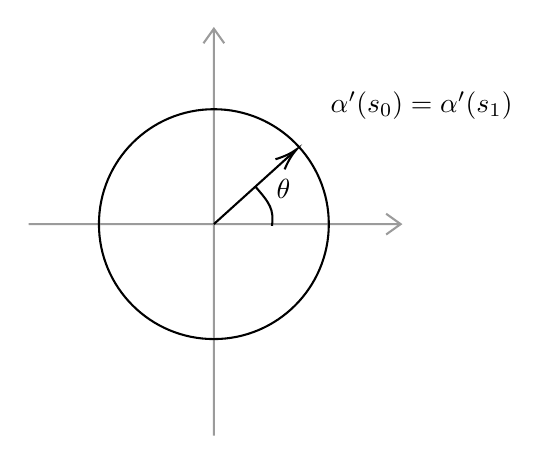
\begin{tikzpicture}[x=0.75pt,y=0.75pt,yscale=-1,xscale=1]
            %uncomment if require: \path (0,300); %set diagram left start at 0, and has height of 300

            %Shape: Axis 2D [id:dp1022754048671688] 
            \draw [color={rgb, 255:red, 155; green, 155; blue, 155 }  ,draw opacity=1 ] (260,143.65) -- (439.2,143.65)(349.2,49.5) -- (349.2,245.5) (432.2,138.65) -- (439.2,143.65) -- (432.2,148.65) (344.2,56.5) -- (349.2,49.5) -- (354.2,56.5)  ;
            %Shape: Circle [id:dp3709466656659819] 
            \draw   (293.83,143.65) .. controls (293.83,113.07) and (318.62,88.28) .. (349.2,88.28) .. controls (379.78,88.28) and (404.58,113.07) .. (404.58,143.65) .. controls (404.58,174.23) and (379.78,199.03) .. (349.2,199.03) .. controls (318.62,199.03) and (293.83,174.23) .. (293.83,143.65) -- cycle ;
            %Straight Lines [id:da5170953335810249] 
            \draw    (349.2,143.65) -- (387.72,108.84) ;
            \draw [shift={(389.2,107.5)}, rotate = 137.89] [color={rgb, 255:red, 0; green, 0; blue, 0 }  ][line width=0.75]    (10.93,-3.29) .. controls (6.95,-1.4) and (3.31,-0.3) .. (0,0) .. controls (3.31,0.3) and (6.95,1.4) .. (10.93,3.29)   ;
            %Curve Lines [id:da2909694502676827] 
            \draw    (377.2,144.5) .. controls (378.2,136.5) and (376.2,133.58) .. (369.2,125.58) ;

            % Text Node
            \draw (404,78.4) node [anchor=north west][inner sep=0.75pt]    {$\alpha '( s_{0}) =\alpha '( s_{1})$};
            % Text Node
            \draw (378,120.4) node [anchor=north west][inner sep=0.75pt]    {$\theta $};


        \end{tikzpicture}
    \end{center}
    As we have discussed in the lecture, if $\theta$ is the angle between $t(s)$ and a fixed direction
    \[k=\frac{\dd \theta}{\dd s}.\]
    Hence, we can consider a function:
    $$
        \theta(s)=\int_{s_0}^s k(s) \dd s .
    $$
    By assumption, $\theta(s)$ is non-decreasing $(k \geq 0)$
    and $\theta\left(s_0\right)=0$
    \[\theta\left(s_0+L\right)=\int_{s_0}^{s_0+L} k(s) \dd s=2 \pi.\]
    (Fact: for a simple closed curve in $\mathbb{R}^2, \int_c k \dd s=2 \pi$)

    Since for each unit vector $\alpha^{\prime}(s)$, we have a unique $\theta(s)\in [0,2 \pi)$
    $$
        \alpha^{\prime}\left(s_0\right)=\alpha^{\prime}\left(s_1\right) \Rightarrow \theta\left(s_0\right)=\theta\left(s_1\right)\in [0,2 \pi) \quad\left(\because \theta:\left[s_0, s_0+L\right) \stackrel{\nearrow }{\rightarrow}[0.2 \pi)\right).
    $$
    But \[s_0<s_1 \Rightarrow \theta(s_0)= \text{constant on } \left[s_0,s_1\right]\]
    \[\Rightarrow \alpha^{\prime}(s)=\text{constant on} \left[s_0 , s_1\right] ,~\alpha'(s)=\alpha^{\prime}(s_0)\]
    \[\Rightarrow \quad \int_{s_0}^{s_1}\left\langle\alpha^{\prime}(s), \vec{n}_0\right\rangle d s=\langle\alpha(s_1)-\alpha(s_0),\vec{n}_0\rangle=h(s_1).\]
    This contradicts $h(s_1)<0$
\end{proof}
\subsubsection*{Further explanation of the four-vertex theorem(sketch)}
Let $L$ be the line passing through $\alpha(s_0)$ and $\alpha(s_1)$, and $\alpha(s_0)$ is a $k_{\min}$ point and $\alpha(s_1)$ is a $k_{\max}$ point.

\textbf{Claim 1}: It can't happen that all points lie on the same side of $L$, \ie\ the configuration in this illustration is impossible.
\begin{center}
    


\tikzset{every picture/.style={line width=0.75pt}} %set default line width to 0.75pt        

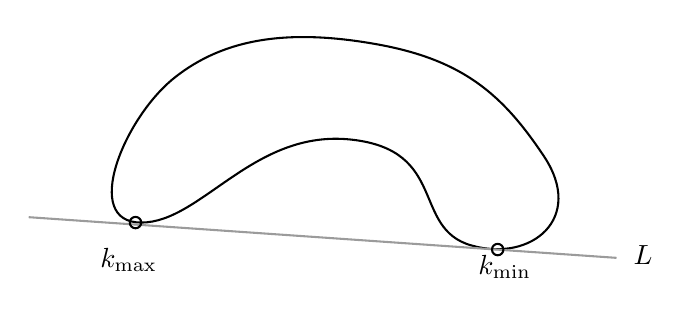
\begin{tikzpicture}[x=0.75pt,y=0.75pt,yscale=-1,xscale=1]
%uncomment if require: \path (0,300); %set diagram left start at 0, and has height of 300

%Shape: Polygon Curved [id:ds49662987101642475] 
\draw   (213,87) .. controls (237.2,67.6) and (268.4,63.2) .. (310.2,70.6) .. controls (352,78) and (371.2,94.6) .. (391.2,124.6) .. controls (411.2,154.6) and (385.13,175.92) .. (356.2,167.6) .. controls (327.27,159.28) and (345.2,121.6) .. (298.2,116.6) .. controls (251.2,111.6) and (226.2,156.6) .. (197.2,156.6) .. controls (168.2,156.6) and (188.8,106.4) .. (213,87) -- cycle ;
%Straight Lines [id:da34126944987507324] 
\draw [color={rgb, 255:red, 155; green, 155; blue, 155 }  ,draw opacity=1 ]   (143,154) -- (426.2,173.6) ;
%Shape: Circle [id:dp14005809041388972] 
\draw   (191.7,156.6) .. controls (191.7,155.08) and (192.93,153.85) .. (194.45,153.85) .. controls (195.97,153.85) and (197.2,155.08) .. (197.2,156.6) .. controls (197.2,158.12) and (195.97,159.35) .. (194.45,159.35) .. controls (192.93,159.35) and (191.7,158.12) .. (191.7,156.6) -- cycle ;
%Shape: Circle [id:dp3958585671594774] 
\draw   (366.2,169.6) .. controls (366.2,168.08) and (367.43,166.85) .. (368.95,166.85) .. controls (370.47,166.85) and (371.7,168.08) .. (371.7,169.6) .. controls (371.7,171.12) and (370.47,172.35) .. (368.95,172.35) .. controls (367.43,172.35) and (366.2,171.12) .. (366.2,169.6) -- cycle ;

% Text Node
\draw (358.2,171) node [anchor=north west][inner sep=0.75pt]    {$k_{\min}$};
% Text Node
\draw (176,167.4) node [anchor=north west][inner sep=0.75pt]    {$k_{\max}$};
% Text Node
\draw (433,166.4) node [anchor=north west][inner sep=0.75pt]    {$L$};


\end{tikzpicture}
\end{center}
(Reason: simple closed + convexity $\Rightarrow \theta(s)
$ is increasing on $[0,2\pi]$, the same argument as the previous page.) 
This implies that there must be points on both sides of $L$. 

\textbf{Claim }: No other points of $C$ meet $L$. 
\begin{center}
    


\tikzset{every picture/.style={line width=0.75pt}} %set default line width to 0.75pt        

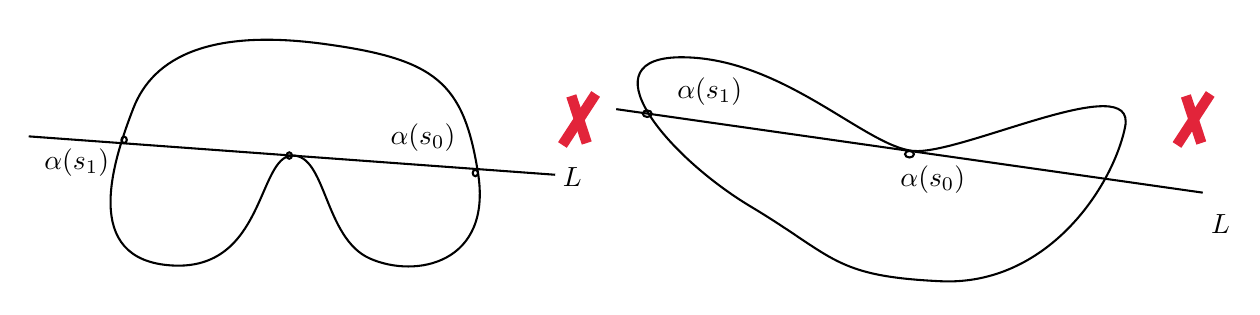
\begin{tikzpicture}[x=0.75pt,y=0.75pt,yscale=-0.9,xscale=0.9]
%uncomment if require: \path (0,300); %set diagram left start at 0, and has height of 300

%Shape: Polygon Curved [id:ds3071120878409017] 
\draw   (86.68,128.1) .. controls (97.49,100.08) and (128.53,85.42) .. (188.61,93.54) .. controls (248.68,101.67) and (263.51,114.09) .. (271.23,162.66) .. controls (278.95,211.23) and (237.88,219.31) .. (213.32,208.43) .. controls (188.76,197.55) and (189.99,152.5) .. (171.62,153.32) .. controls (153.25,154.14) and (156.95,214.97) .. (107.53,212.17) .. controls (58.11,209.36) and (75.87,156.12) .. (86.68,128.1) -- cycle ;
%Straight Lines [id:da6805550926024335] 
\draw    (30.7,143.05) -- (312.54,163.6) ;
%Shape: Ellipse [id:dp5838511313323707] 
\draw   (168.76,153.32) .. controls (168.76,154.28) and (169.4,155.05) .. (170.19,155.05) .. controls (170.98,155.05) and (171.62,154.28) .. (171.62,153.32) .. controls (171.62,152.37) and (170.98,151.59) .. (170.19,151.59) .. controls (169.4,151.59) and (168.76,152.37) .. (168.76,153.32) -- cycle ;
%Shape: Ellipse [id:dp38388215977449014] 
\draw   (80.35,144.92) .. controls (80.35,145.88) and (80.99,146.65) .. (81.78,146.65) .. controls (82.57,146.65) and (83.21,145.88) .. (83.21,144.92) .. controls (83.21,143.97) and (82.57,143.19) .. (81.78,143.19) .. controls (80.99,143.19) and (80.35,143.97) .. (80.35,144.92) -- cycle ;
%Shape: Ellipse [id:dp36329266716854014] 
\draw   (268.37,162.66) .. controls (268.37,163.62) and (269.01,164.39) .. (269.8,164.39) .. controls (270.59,164.39) and (271.23,163.62) .. (271.23,162.66) .. controls (271.23,161.71) and (270.59,160.93) .. (269.8,160.93) .. controls (269.01,160.93) and (268.37,161.71) .. (268.37,162.66) -- cycle ;
%Shape: Right Angle [id:dp5810238140777244] 
\draw  [color={rgb, 255:red, 226; green, 36; blue, 58 }  ,draw opacity=1 ][line width=3.75]  (321.19,121.39) -- (325.31,134.01) -- (316.42,147.66) ;
%Shape: Right Angle [id:dp947959045950229] 
\draw  [color={rgb, 255:red, 226; green, 36; blue, 58 }  ,draw opacity=1 ][line width=3.75]  (329.43,146.61) -- (325.31,133.99) -- (334.2,120.35) ;

%Shape: Polygon Curved [id:ds8274619497323568] 
\draw   (417.24,180.63) .. controls (371.98,153.54) and (327.65,100.02) .. (381.22,100.7) .. controls (434.78,101.37) and (478.59,148.3) .. (504.05,150.83) .. controls (529.51,153.35) and (624.11,106.12) .. (617.64,137.96) .. controls (611.18,169.79) and (576.08,223.31) .. (518.82,220.6) .. controls (461.56,217.89) and (462.49,207.73) .. (417.24,180.63) -- cycle ;
%Straight Lines [id:da11395275306166774] 
\draw    (345.2,128.47) -- (659.2,173.18) ;
%Shape: Ellipse [id:dp10283110241696836] 
\draw   (499.8,152.59) .. controls (499.8,151.61) and (500.87,150.83) .. (502.2,150.83) .. controls (503.53,150.83) and (504.6,151.61) .. (504.6,152.59) .. controls (504.6,153.56) and (503.53,154.35) .. (502.2,154.35) .. controls (500.87,154.35) and (499.8,153.56) .. (499.8,152.59) -- cycle ;
%Shape: Ellipse [id:dp5551670999500844] 
\draw   (359.42,130.91) .. controls (359.42,129.94) and (360.5,129.15) .. (361.82,129.15) .. controls (363.15,129.15) and (364.22,129.94) .. (364.22,130.91) .. controls (364.22,131.88) and (363.15,132.67) .. (361.82,132.67) .. controls (360.5,132.67) and (359.42,131.88) .. (359.42,130.91) -- cycle ;
%Shape: Right Angle [id:dp5407499071484163] 
\draw  [color={rgb, 255:red, 226; green, 36; blue, 58 }  ,draw opacity=1 ][line width=3.75]  (650.19,121.39) -- (654.31,134.01) -- (645.42,147.66) ;
%Shape: Right Angle [id:dp08794142716571418] 
\draw  [color={rgb, 255:red, 226; green, 36; blue, 58 }  ,draw opacity=1 ][line width=3.75]  (658.43,146.61) -- (654.31,133.99) -- (663.2,120.35) ;


% Text Node
\draw (37.41,147.77) node [anchor=north west][inner sep=0.75pt]    {$\alpha ( s_{1})$};
% Text Node
\draw (222.75,134.5) node [anchor=north west][inner sep=0.75pt]    {$\alpha ( s_{0})$};
% Text Node
\draw (315,158.05) node [anchor=north west][inner sep=0.75pt]    {$L$};
% Text Node
\draw (376.27,110) node [anchor=north west][inner sep=0.75pt]    {$\alpha ( s_{1})$};
% Text Node
\draw (495.71,157.24) node [anchor=north west][inner sep=0.75pt]    {$\alpha ( s_{0})$};
% Text Node
\draw (662,183.05) node [anchor=north west][inner sep=0.75pt]    {$L$};


\end{tikzpicture}
\end{center}
(Reason: same as Claim 1.) Hence, Claim 1 + Claim 2$\Rightarrow$ 
\begin{center}
    


\tikzset{every picture/.style={line width=0.75pt}} %set default line width to 0.75pt        

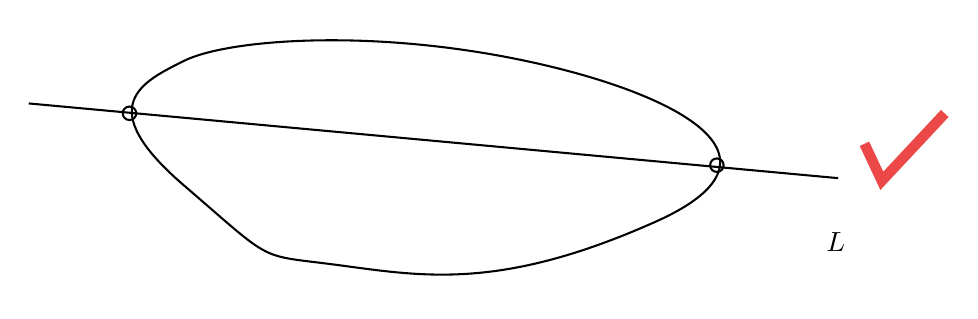
\begin{tikzpicture}[x=0.75pt,y=0.75pt,yscale=-1,xscale=1]
%uncomment if require: \path (0,300); %set diagram left start at 0, and has height of 300

%Shape: Polygon Curved [id:ds7702382474499099] 
\draw   (140,53) .. controls (160,43) and (225.2,37.5) .. (297.2,51.5) .. controls (369.2,65.5) and (441.2,97.5) .. (367.2,130.5) .. controls (293.2,163.5) and (255.95,156.97) .. (215.2,151.5) .. controls (174.45,146.03) and (184.8,151.5) .. (140,113) .. controls (95.2,74.5) and (120,63) .. (140,53) -- cycle ;
%Straight Lines [id:da6986447532784184] 
\draw    (65.2,73.5) -- (455.2,109.5) ;
%Shape: Circle [id:dp736182231164852] 
\draw   (393.5,103.25) .. controls (393.5,101.46) and (394.96,100) .. (396.75,100) .. controls (398.54,100) and (400,101.46) .. (400,103.25) .. controls (400,105.04) and (398.54,106.5) .. (396.75,106.5) .. controls (394.96,106.5) and (393.5,105.04) .. (393.5,103.25) -- cycle ;
%Shape: Circle [id:dp35739367600902905] 
\draw   (110.5,78.25) .. controls (110.5,76.46) and (111.96,75) .. (113.75,75) .. controls (115.54,75) and (117,76.46) .. (117,78.25) .. controls (117,80.04) and (115.54,81.5) .. (113.75,81.5) .. controls (111.96,81.5) and (110.5,80.04) .. (110.5,78.25) -- cycle ;
%Shape: Right Angle [id:dp7746325035072514] 
\draw  [color={rgb, 255:red, 236; green, 72; blue, 72 }  ,draw opacity=1 ][line width=3.75]  (506.56,78.34) -- (476.22,110.79) -- (467.86,92.95) ;

% Text Node
\draw (448,134.4) node [anchor=north west][inner sep=0.75pt]    {$L$};


\end{tikzpicture}
\end{center}
\textbf{Claim 3}: $\exists$ a third and a fourth vertex. (See the proof)

\begin{exercise}
    Let $\alpha(s)=\left(x(s),y(s)\right)$ be a simple closed curve in 
    $\mathbb{R}^2$. Let $\tilde{\alpha}(s)$ be the image of $\alpha(s)$ 
    under stereographic projection. Show that if $\alpha(s_0)$ is a vertex 
    of $\alpha(s)$, then $\tilde{\alpha}(s_0)$ has vanishing torsion.
\end{exercise}
\begin{example}
    \hfill
    \begin{itemize}
        \item The circle with radius $r$ and curvature $k=\frac{1}{r}$ has infinitely many vertices.
        \begin{center}
            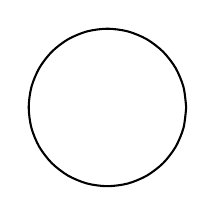
\begin{tikzpicture}
                \draw[smooth,domain=0:360,variable=\t]
                plot ({cos(\t)},{sin(\t)});
            \end{tikzpicture}
        \end{center}
        \item An ellipse has four vertices.
        \begin{center}
            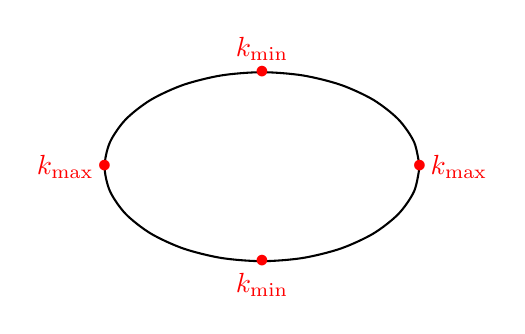
\begin{tikzpicture}
                \draw[smooth,domain=0:360,variable=\t]
                plot ({2*cos(\t)},{1.2*sin(\t)});
                \draw[red] (2,0) node {$\bullet$};
                \draw[red] (-2,0) node {$\bullet$};
                \draw[red] (0,1.2) node {$\bullet$};
                \draw[red] (0,-1.2) node {$\bullet$};
                \draw[red] (2.5,0) node {$k_{\max}$};
                \draw[red] (-2.5,0) node {$k_{\max}$};
                \draw[red] (0,1.5) node {$k_{\min}$};
                \draw[red] (0,-1.5) node {$k_{\min}$};
            \end{tikzpicture}
        \end{center}
        \item Although this is nonconvex, it has more than four vertices.
        \begin{center}
            


\tikzset{every picture/.style={line width=0.75pt}} %set default line width to 0.75pt        

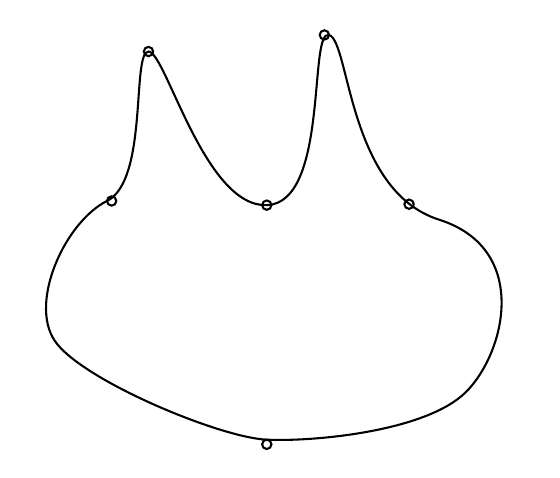
\begin{tikzpicture}[x=0.75pt,y=0.75pt,yscale=-1,xscale=1]
%uncomment if require: \path (0,300); %set diagram left start at 0, and has height of 300

%Shape: Polygon Curved [id:ds4426374143902496] 
\draw   (276.2,124.7) .. controls (296.2,114.7) and (288,52.96) .. (296.2,52.7) .. controls (304.4,52.44) and (323.14,127.79) .. (353.2,126.7) .. controls (383.26,125.61) and (373.2,41.7) .. (383.2,44.7) .. controls (393.2,47.7) and (392.2,119.7) .. (436.2,133.7) .. controls (480.2,147.7) and (468.2,197.7) .. (449.2,216.7) .. controls (430.2,235.7) and (376.11,240.74) .. (353.2,239.7) .. controls (330.29,238.66) and (263.5,210.75) .. (251,192) .. controls (238.5,173.25) and (256.2,134.7) .. (276.2,124.7) -- cycle ;
%Shape: Circle [id:dp24475690948115414] 
\draw   (350.95,241.95) .. controls (350.95,240.71) and (351.96,239.7) .. (353.2,239.7) .. controls (354.44,239.7) and (355.45,240.71) .. (355.45,241.95) .. controls (355.45,243.19) and (354.44,244.2) .. (353.2,244.2) .. controls (351.96,244.2) and (350.95,243.19) .. (350.95,241.95) -- cycle ;
%Shape: Circle [id:dp6463699176238631] 
\draw   (293.95,52.7) .. controls (293.95,51.46) and (294.96,50.45) .. (296.2,50.45) .. controls (297.44,50.45) and (298.45,51.46) .. (298.45,52.7) .. controls (298.45,53.94) and (297.44,54.95) .. (296.2,54.95) .. controls (294.96,54.95) and (293.95,53.94) .. (293.95,52.7) -- cycle ;
%Shape: Circle [id:dp22246063551555872] 
\draw   (419.5,126.25) .. controls (419.5,125.01) and (420.51,124) .. (421.75,124) .. controls (422.99,124) and (424,125.01) .. (424,126.25) .. controls (424,127.49) and (422.99,128.5) .. (421.75,128.5) .. controls (420.51,128.5) and (419.5,127.49) .. (419.5,126.25) -- cycle ;
%Shape: Circle [id:dp15960337604147457] 
\draw   (350.95,126.7) .. controls (350.95,125.46) and (351.96,124.45) .. (353.2,124.45) .. controls (354.44,124.45) and (355.45,125.46) .. (355.45,126.7) .. controls (355.45,127.94) and (354.44,128.95) .. (353.2,128.95) .. controls (351.96,128.95) and (350.95,127.94) .. (350.95,126.7) -- cycle ;
%Shape: Circle [id:dp04023095022735057] 
\draw   (378.7,44.7) .. controls (378.7,43.46) and (379.71,42.45) .. (380.95,42.45) .. controls (382.19,42.45) and (383.2,43.46) .. (383.2,44.7) .. controls (383.2,45.94) and (382.19,46.95) .. (380.95,46.95) .. controls (379.71,46.95) and (378.7,45.94) .. (378.7,44.7) -- cycle ;
%Shape: Circle [id:dp5025388061962088] 
\draw   (276.2,124.7) .. controls (276.2,123.46) and (277.21,122.45) .. (278.45,122.45) .. controls (279.69,122.45) and (280.7,123.46) .. (280.7,124.7) .. controls (280.7,125.94) and (279.69,126.95) .. (278.45,126.95) .. controls (277.21,126.95) and (276.2,125.94) .. (276.2,124.7) -- cycle ;




\end{tikzpicture}
        \end{center}
    \end{itemize}
\end{example}
\begin{proof}[Proof of \cref{thm:four-vertex theorem}]
    Let $\alpha(s)$ be parametrized by arclength. First, since the curvature
    $k(s)$ is a continuous function on $I$, it must have maximum and 
    minimum, at which $k'(s)=0$, \ie\ $\alpha(s)$ has at least $2$ vertices.
    Let $\alpha(s_0)$ be a $k_{\min}$ point, $\alpha(s_1)$ be a $k_{\max}$ 
    point. Consider a line $l$ connecting $\alpha(s_0)$ and $\alpha(s_1)$. For convenience, we assume line $l$ coincides with $x$-axis.
    \begin{center}
        


\tikzset{every picture/.style={line width=0.75pt}} %set default line width to 0.75pt        

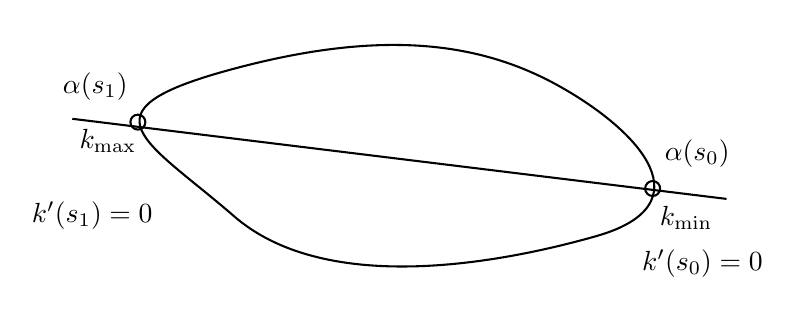
\begin{tikzpicture}[x=0.75pt,y=0.75pt,yscale=-1,xscale=1]
%uncomment if require: \path (0,300); %set diagram left start at 0, and has height of 300

%Shape: Polygon Curved [id:ds06277821638958292] 
\draw   (137.2,40.6) .. controls (210.2,20.6) and (258.2,26.6) .. (297.2,48.6) .. controls (336.2,70.6) and (367.2,105.6) .. (314.2,120.6) .. controls (261.2,135.6) and (182.2,147.6) .. (140,111) .. controls (97.8,74.4) and (64.2,60.6) .. (137.2,40.6) -- cycle ;
%Straight Lines [id:da7129598017341983] 
\draw    (62,64) -- (377.2,102.6) ;
%Shape: Circle [id:dp20289567099794015] 
\draw   (90,65.6) .. controls (90,63.61) and (91.61,62) .. (93.6,62) .. controls (95.59,62) and (97.2,63.61) .. (97.2,65.6) .. controls (97.2,67.59) and (95.59,69.2) .. (93.6,69.2) .. controls (91.61,69.2) and (90,67.59) .. (90,65.6) -- cycle ;
%Shape: Circle [id:dp11839975645101264] 
\draw   (338,97.6) .. controls (338,95.61) and (339.61,94) .. (341.6,94) .. controls (343.59,94) and (345.2,95.61) .. (345.2,97.6) .. controls (345.2,99.59) and (343.59,101.2) .. (341.6,101.2) .. controls (339.61,101.2) and (338,99.59) .. (338,97.6) -- cycle ;

% Text Node
\draw (56,40.4) node [anchor=north west][inner sep=0.75pt]    {$\alpha ( s_{1})$};
% Text Node
\draw (346,72.4) node [anchor=north west][inner sep=0.75pt]    {$\alpha ( s_{0})$};
% Text Node
\draw (64,67.4) node [anchor=north west][inner sep=0.75pt]    {$k_{\max}$};
% Text Node
\draw (343.6,104.6) node [anchor=north west][inner sep=0.75pt]    {$k_{\min}$};
% Text Node
\draw (41,102.4) node [anchor=north west][inner sep=0.75pt]    {$k'( s_{1}) =0$};
% Text Node
\draw (335,125.4) node [anchor=north west][inner sep=0.75pt]    {$k'( s_{0}) =0$};


\end{tikzpicture}
    \end{center}

    The First observation is: on $l$, there is no other point of $\alpha(s)$. 
    Hence, $\alpha(s)$ is divided into two pieces. If not, assume 
    $\alpha(s_2)$ is a third point, and W.L.O.G. assume $k'(s_2)=0$. 
    The tangent line at $\alpha(s_2)$ must be the same as $l$. Since the 
    curve $\alpha$ is convex, the whole curve $\alpha(s)$ must lie on the 
    same side of $l$. This forces the tangent lines of $\alpha(s_0)$ and 
    $\alpha(s_1)$ can only be $l$. But $\alpha(s_0)$ is a $k_{\min}$ point
    and $\alpha(s_1)$ is a $k_{\max}$ point, which implies $k(s_0)=k(s_1)=0$. Therefore, $k\equiv 0$ on $\alpha$, a contradiction.

    \begin{center}
        


\tikzset{every picture/.style={line width=0.75pt}} %set default line width to 0.75pt        

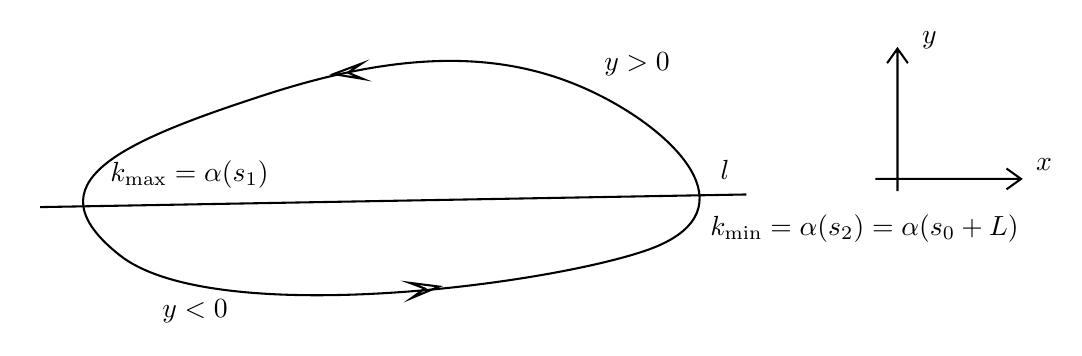
\begin{tikzpicture}[x=0.75pt,y=0.75pt,yscale=-1,xscale=1]
%uncomment if require: \path (0,300); %set diagram left start at 0, and has height of 300

%Shape: Polygon Curved [id:ds06277821638958292] 
\draw   (135.27,41.84) .. controls (207.3,18.59) and (255.52,22.43) .. (295.47,42.66) .. controls (335.42,62.89) and (368.74,100.23) .. (316.47,117.6) .. controls (264.19,134.96) and (107.7,154.16) .. (63.9,119.49) .. controls (20.1,84.82) and (63.24,65.1) .. (135.27,41.84) -- cycle ;
%Straight Lines [id:da7129598017341983] 
\draw    (25.55,96.35) -- (365.86,90.26) ;
\draw   (181.2,34.6) -- (166.97,32.25) -- (180.47,27.18) -- (173.9,31.57) -- cycle ;
\draw   (203.5,132.81) -- (217.81,134.63) -- (204.51,140.2) -- (210.9,135.57) -- cycle ;
%Shape: Axis 2D [id:dp6987088884625297] 
\draw  (428,82.77) -- (498.2,82.77)(438.67,20) -- (438.67,88.6) (491.2,77.77) -- (498.2,82.77) -- (491.2,87.77) (433.67,27) -- (438.67,20) -- (443.67,27)  ;

% Text Node
\draw (296,20.4) node [anchor=north west][inner sep=0.75pt]    {$y >0$};
% Text Node
\draw (83,139.4) node [anchor=north west][inner sep=0.75pt]    {$y< 0$};
% Text Node
\draw (347,98.4) node [anchor=north west][inner sep=0.75pt]    {$k_{\min} =\alpha ( s_{2}) =\alpha ( s_{0} +L)$};
% Text Node
\draw (58,72.4) node [anchor=north west][inner sep=0.75pt]    {$k_{\max} =\alpha ( s_{1})$};
% Text Node
\draw (504,71.4) node [anchor=north west][inner sep=0.75pt]    {$x$};
% Text Node
\draw (449,10.4) node [anchor=north west][inner sep=0.75pt]    {$y$};
% Text Node
\draw (352,72.4) node [anchor=north west][inner sep=0.75pt]    {$l$};


\end{tikzpicture}
    \end{center}

    Next, we look for the third vertex. If $\alpha(s)$ has only two vertices
    at $\alpha(s_0)$ and $\alpha(s_1)$, then from $s_0$ to $s_1$, $k'(s)>0$ 
    and from $s_1$ to $s_0+L$, $k'(s)<0$
    \[\Rightarrow y\cdot k'(s)\ge 0,~\forall s\]
    \[\Rightarrow 0<\int_\alpha y\cdot k'(s)\dd s=-\int_\alpha y'(s)k\dd s.\]
    Note that if 
    \[\alpha(s)=\left(x(s),y(s)\right), t(s)=\alpha'(s)\left(x'(s),y'(s)\right).\]
    \[t'(s)=\left(x''(s),y''(s)\right)=k \vec{n}=k(-y',x')\Rightarrow -k'(s)k=x''\]
    \[\therefore \int_\alpha y' k\dd s=\int_\alpha x'' \dd s=0.\]
    A contradiction!. Hence, there must be a third vertex, say $\alpha(s_2)$, at which $k'(s_2)=0$.

    Note that $k'(s)$ changes its sign at vertices, so the number of 
    vertices must be even. Then there are at least $4$ vertices.
\end{proof}
\begin{remark}
    The proof of the four-vertex theorem for non-convex 
    case can be found in Montiel-Ros's book Chapter 9.6. 
    (4-vertex theorem for space curves: simple closed curve on a convex surface has at least four points with vanishing torsion.)
\end{remark}
\subsection{Minkowski problem(1-d)}
\begin{theorem}[1-d Minkowski problem]
    \label{thm: Minkowski problem}
    Given a periodic, strictly positive function k, satisfying the following condition:
    \[\int_0^{2\pi}\frac{\cos \theta}{k}\dd \theta=
    \int_0^{2\pi}\frac{\sin \theta}{k}\dd \theta=0
    .\]
    There is an oval in 
    $\mathbb{R}^2$ (\ie\ simple closed strictly convex curve) such that 
    the curvature function is $k$. 
\end{theorem}
\begin{definition}
    A plane curve $\alpha(t)$ is strictly convex iff $\alpha(t)$ is convex 
    and at each point, the tangent line meets with $\alpha(t)$ at only 
    one point.
\end{definition}
\begin{proposition}
    A simple closed curve is strictly convex iff with inward unit normal 
    vector field, the curvature function $k>0$. 
\end{proposition}
\textbf{Minkowski problem}: Given a strictly positive, periodic function
$k$, does there exist a simple closed convex curve $\alpha$ with $k$
as the curvature function?
\begin{remark}
    This is a prescribed curvature problem. There are a lot of similar 
    questions in geometry. Such problems are usually related to solving
    certain P.D.E.
\end{remark}
Let's derive a differential equation for the above problem. Let $\alpha$ be 
a strictly convex curve, then $k>0$, and we can use the angle parameter $\theta$, \ie\ 
\[\frac{\dd\theta}{\dd s}=k,~\frac{\dd s}{\dd \theta}=\frac{1}{k} \]
\begin{center}
    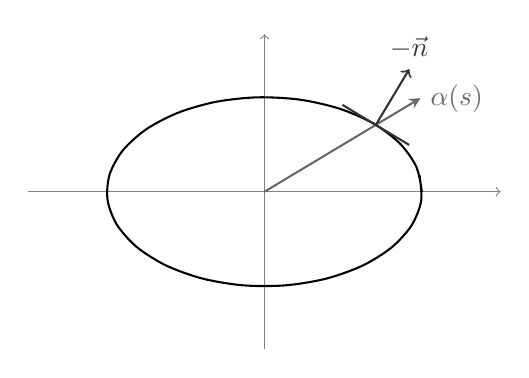
\begin{tikzpicture}
        \draw[black!50, thin, ->] (0, -2) -- (0, 2) ;
        \draw[black!50, thin, ->] (-3, 0) -- (3, 0) ;
        \draw[smooth,domain=0:370,variable=\t]
        plot ({2*cos(\t)},{1.2*sin(\t)});
        \draw[->,>=stealth,black!60](0,0)to({1.4*2*cos(45)},{1.4*1.2*sin(45)}) node[right]{$\alpha(s)$};
        \draw[smooth,domain=-0.3:0.3,variable=\t,black!80]
        plot ({2*cos(45)+2*(-sin(45))*\t},{1.2*sin(45)+1.2*cos(45)*\t});
        \draw[smooth,domain=0:0.5,variable=\t,black!80,->]
        plot ({2*cos(45)+1.2*cos(45)*\t},{1.2*sin(45)+2*(sin(45))*\t})
        node[above] {$-\vec{n}$};
    \end{tikzpicture}
\end{center}
Consider a function
\[
    h(s)=-\left<\alpha(s),\vec{n}(s)\right>\text{ support function}.
\]
(Recall $\int_C h(s)\dd s=2\cdot\mathrm{Area}$).\\
Clearly $h(0)=h(2\pi)$ if
 we use 
 $h(\theta)=-\langle\alpha\left(s(\theta)\right),\vec{n}\left(s(\theta)\right)\rangle$. 
 \begin{align*}
    h'(\theta)&=-\langle \alpha'(s)\frac{\dd s}{\dd\theta},\vec{n}(s)\rangle
    -\langle \alpha(\theta),\frac{\dd \vec{n}}{\dd s}\frac{\dd s}{\dd \theta}\rangle\\
    &=-\langle \alpha(\theta),-k\cdot\vec{t}\cdot\frac{1}{k}\rangle =\langle\alpha(\theta),\vec{t}\left(s(\theta)\right)\rangle
.\end{align*}
Hence, $h'(0)=h'(2\pi)$.

We also conclude that
\begin{align*}
    \alpha(\theta)&=\langle \alpha(\theta), \vec{t}\rangle \cdot \vec{t}
    +\langle \alpha(\theta), \vec{n}\rangle \cdot \vec{n}\\
    &=h'(\theta)\vec{t}-h(\theta)\vec{n}
,\end{align*}
\ie\ the curve is determined by the support function $h$. \\
$\left(\alpha(s)=h'(s)\dfrac{\dd s}{\dd \theta}\vec{t}-h(s)\vec{n}=h'(s)\dfrac{1}{k}\vec{t}-h(s)\vec{n}\right)$
\begin{align*}
    h''(\theta)&=\langle \alpha'(s)\frac{\dd s}{\dd \theta},\vec{t}\rangle
    +\langle \alpha(\theta),\frac{\dd \vec{t}}{\dd s}\frac{\dd s}{\dd \theta}
    \rangle\\
    &=\frac{1}{k}+\langle\alpha(\theta),k\vec{n}\cdot \frac{1}{k}\rangle=\frac{1}{k}-h
.\end{align*}
\ie\ $\boxed{h''(\theta)+h(\theta)=\frac{1}{k}}$.

Hence, if $\alpha(s)=\alpha(\theta)$ is a strictly convex closed curve, the
support function $h(\theta)=-\langle\alpha,\vec{n}\rangle$ satisfies a second
linear o.d.e.
\[h''(\theta)+h=\frac{1}{k}.\]
\textbf{Observation:} If $\exists~h$ that satisfies the equation above.
Note $\theta\in [0,2\pi)$, then
\begin{align*}
    \int_0^{2\pi}\cos\theta\frac{1}{k}\dd \theta&=
    \int_0^{2\pi} \cos\theta\cdot\left(h''\theta+h\right)\dd \theta\\
    &=\int_0^{2\pi}\sin\theta\cdot h'(\theta)+\int_0^{2\pi}\cos \theta \cdot h\\
    &=-\int_0^{2\pi}\cos\theta \cdot h(\theta)+\int_0^{2\pi}\cos\theta \cdot h=0
.\end{align*}
Similarly,
\[\int_0^{2\pi}\sin\theta\cdot\frac{1}{k}\dd \theta=0,\]
\ie\ if $k$ is the curvature of a strictly convex curve, it must satisfy
\[
    \int_0^{2\pi}\cos\theta\cdot\frac{1}{k}\dd \theta
    =\int_0^{2\pi}\sin\theta\cdot\frac{1}{k}\dd \theta
    =0
.\]

In fact, from o.d.e, we can directly construct the solution like this:
\[
    h(\theta)=-\cos\theta \int_0^\theta \frac{\sin \psi}{k}\dd \psi
    +\sin\theta \int_0^\theta \frac{\cos \psi}{k}\dd \psi  
.\]
Recall that $\vec{t}(s)=(\cos\theta,\sin\theta),~\vec{n}(s)=(-\sin \theta,\cos\theta).$
Since
\begin{align*}
    \alpha(\theta)&=h'(\theta)\vec{t}-h(\theta)\vec{n}\\
    &=\left(
        \cos\theta\sin\theta\int_0^\theta\frac{\sin\psi}{k}
        +\cos^2\theta\int_0^\theta\frac{\cos\psi}{k},
        \sin^2\theta\int_0^\theta\frac{\sin\psi}{k}
        +\sin\theta\cos\theta\int_0^\theta\frac{\cos\psi}{k}
    \right)\\
    &\quad-\left( 
        \sin\theta\cos\theta\int_0^\theta\frac{\sin\psi}{k}
        -\sin^2\theta\int_0^\theta\frac{\cos\psi}{k},
        -\cos^2\theta\int_0^\theta\frac{\sin\psi}{k}
        +\sin\theta\cos\theta\int_0^\theta\frac{\cos\psi}{k}
    \right)\\
    &=\left(
        \int_0^\theta\frac{\cos\psi}{k},
        \int_0^\theta\frac{\sin\psi}{k}
    \right)
\end{align*}
$\alpha(s)$ is closed $\Leftrightarrow~h(0)=h(2\pi),~h'(0)=h'(2\pi)
\Leftrightarrow \int_0^{2\pi}\cos\theta\cdot\dfrac{1}{k}\dd \theta
=\int_0^{2\pi}\sin\theta\cdot\dfrac{1}{k}\dd \theta
=0$.
\begin{remark}
    In general (higher dimensional case) solving a similar P.D.E. equation is highly nontrivial!
    
    Cheng-Yau 1976 CPAM: given a $C^{k,\alpha}$ positive function $K$ on the
    sphere $\mathbb{S}^n$ ($k\ge 3$), which satisfies
    \[
    \int_{\mathbb{S}^n}\frac{x_i}{K}\dd V_{\mathbb{S}^n}=0
    ,\]
    where $x_1,x_2,\cdots,x_{n+1}$ are coordinate functions on 
    $\mathbb{S}^n$. 
    Then there is a strictly convex closed 
    hypersurface $M^n \hookrightarrow \mathbb{R}^{n+1}$ such
    that the Gaussian curvature is $K$.
\end{remark} 
